\documentclass[conference]{IEEEtran}
\IEEEoverridecommandlockouts
% The preceding line is only needed to identify funding in the first footnote. If that is unneeded, please comment it out.
\usepackage{cite}
\usepackage{amsmath,amssymb,amsfonts}
\usepackage{algorithmic}
\usepackage{graphicx}
\usepackage{textcomp}
\usepackage{xcolor}
\usepackage{tabularx}

\usepackage{fancyhdr}
\pagestyle{fancy}
\lhead{Michigan Robotic Submarine}
\rhead{\thepage}

\def\BibTeX{{\rm B\kern-.05em{\sc i\kern-.025em b}\kern-.08em
    T\kern-.1667em\lower.7ex\hbox{E}\kern-.125emX}}
    
\begin{document}

\title{Michigan Robotic Submarine}
\author{Emi Yuki, Kathryn Wakevainen, Alexander Steinig, Diego Montemayor, Benjamin Steinig, Shrey Sahgal, \\ Nolan Kuza, Bodee Davis, Kobi Wettstein, Shubh Agrawal, James Leung, Andrew Huston, Vikram Raghu
}

\maketitle
\pagestyle{fancy}
\lhead{Michigan Robotic Submarine}
\rhead{\thepage}

\begin{abstract}
Michigan Robotic Submarine is a student project team at the University of Michigan, now in its second year participating in the RoboNation RoboSub competition. Our autonomous underwater vehicle (AUV), Erie (see figure \ref{fig:sub4}), is a complete overhaul of our previous design with an emphasis on modularity for mounting additional components and maneuverability when operating. We accomplished this by focusing on a one-piece hull as a main body with other mechanisms attaching directly to it. There are three tasks we focused on for this year’s game strategy: the buoy task, gate task, and surfacing task. These tasks informed our design decisions and the team's focus for the past year. The mechanical subteam was responsible for designing the main hull, thruster mounts and electronics chassis. The software subteam designed various custom circuit boards for the electrical system and designed a hydrophone system. They also upgraded their pre-existing system architecture to have more flexibility when running navigational programs, upgraded our deep learning models for detection of multiple objects, and implemented a more advanced computer vision system. We developed more robust testing tools and procedures for off and on board testing which included frequent in-water testing on the University of Michigan campus.
\end{abstract}

\section{Competition Strategy}
As a second year team, this year will be the first time that the Michigan Robotic Submarine team is participating in the in-person competition. As such, the team’s main focus was on creating a reliable system that could complete tasks outside of our primary testing environments. In order to accomplish this, we designed and built our new submarine, Erie, to overcome the shortcomings of our previous vehicle, Huron. In particular, Huron posed difficulties in producing the desired movements during testing due to its profile and weight distribution, which made it difficult to test our algorithms' effectiveness. In terms of the competition, Huron's lack of reliable mobility was problematic because competing in-person requires more precision for locating and completing tasks. This informed our mechanical design criteria as we sought to make Erie more maneuverable. On the software subteam, we decided to focus on creating a more robust computer vision system and designated our hydrophone system as a stretch goal. As such, we centered our attention on tasks with large visual components such as the Choose Your Side (Gate) and Make the Grade (Buoy) tasks with the Cash or Smash (Surfacing) task as a reach goal.

\subsection{Choose Your Side (Gate)}\label{AA}
Our main priority was developing the software to consistently complete the gate task, as it is required to qualify for the competition. Because the gate's side posts consist of bright, straight lines which stand out underwater, the gate is easily identifiable using computer vision. As such, we rely on a deep learning model to visually identify the gate to inform our navigational algorithm on the heading of the gate relative to our AUV. While we created a model which identified the gate fairly accurately, we noticed while in-water testing that the model had biases that made it difficult to detect the gate from certain angles or depths. In response, we made an effort to collect more diverse image sets with which we trained our model. Since we already had fairly accurate identification of the gate, we had the bandwidth to add detection of the bootlegger and G-man images for the style points. Our vision system is limited by the GPU performance so we also adjusted our navigation algorithm to accommodate potential latency in the identification of the gate.


\subsection{Make the Grade (Buoy)}\label{AA}
The second task we focused on was bumping the buoy. This was a realistic goal for the team since the systems and general navigation needed for the task are similar to the systems needed to achieve the gate task as they both involve centering the AUV upon visually-detected objects. The first challenge was detecting when the AUV has actually bumped the buoy as we lose visual range of it before the AUV touches it. We decided to use the output from our Attitude and Heading Reference System (AHRS) as we attribute abnormalities in our movement to the collision with the buoy. The second challenge was locating the buoy. In order to accomplish this, we added a camera to the bottom of Erie. We then created a new vision system for identifying the edges of the path marker which we can use to calculate the AUV's relative heading. We can then use the heading to navigate to the buoy task from the gate task. While there was added complexity, we expected this task to be doable given the framework we had started developing in the previous year and our experience in developing vision systems.

\begin{figure}[htbp]
    \centerline{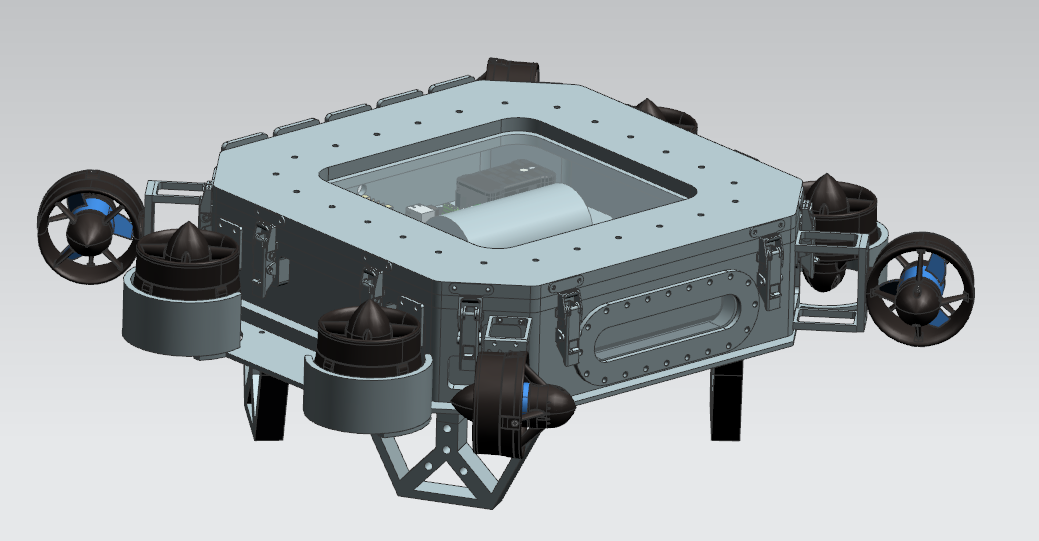
\includegraphics[scale=0.35]{images/sub4.PNG}}
    \caption{CAD of our 2021-2022 AUV, Erie.}
    \label{fig:sub4}
\end{figure}

\subsection{Cash or Smash (Surfacing)}\label{AA}
This last task was a smaller focus for the team, as the acoustic navigation needed to locate this task is more complex and less developed than our vision system. Our hydrophone system made progress as we created and tested custom band-path filters for filtering the input received from our hydrophones. We would like to be able to accomplish tasks related to the pinger, which tend to have higher point values. However, the main focus for the team has been the vision system, as they are needed to complete the qualifying task. Since the gate and buoy tasks are attempted first, there is no detriment to the team attempting the surfacing task. Surfacing within the octagon would yield us more points, but even if the attempt is unsuccessful, there are no other tasks that we would need to complete.


\section{Design Creativity}

\subsection{Mechanical}
This year, our mechanical team primarily focused on redesigning the hull of our AUV. After testing with our previous sub (Huron) extensively, we identified several clear points of improvement that should be made when designing the new hull. Namely, we prioritized camera visibility, leak-proof reliability, electronics accessibility, and maneuverability. Increasing camera visibility entailed eliminating the use of epoxy to aid in sealing the hull, which often obscured part of the camera's field of view. To do this, we implemented a dual face seal o ring system at both the interface between the front window and hull and the interface between the top window and hull. We also sealed the gap between the lid and main hull with an o-ring extending around the outside of the top of the main hull. This dramatically decreased the chance of our sub leaking from last year's design and, in turn, allowed us to avoid using epoxy at any of the sealing points, which improved camera visibility


The main enclosure on Huron was a cylinder sealed on either side by end caps with circumferential o-rings. The only way to access the electrical components was to remove one of the end caps, which was fairly laborious. Our new hull design consists of a large rectangular compartment connected to a lid via hinges on one side of the vehicle in figure \ref{fig:sub6}. When the lid is lowered in the closed position, latches around the outside of the sub are closed to ensure that the lid and hull form a tight seal.

\begin{figure}[htbp]
    \centerline{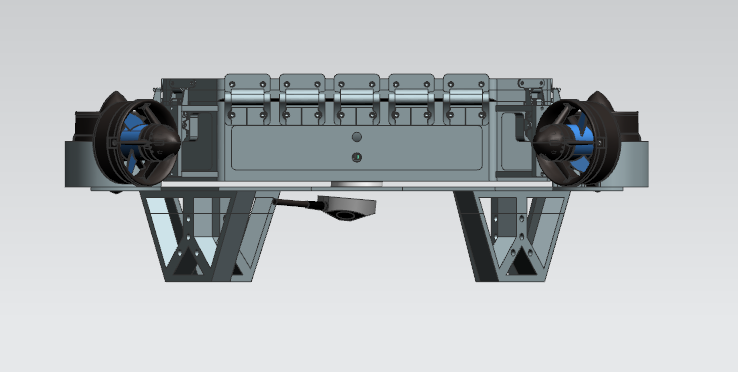
\includegraphics[scale=0.5]{images/sub6.PNG}}
    \caption{CAD of the hinges which connect the lid to the hull.}
    \label{fig:sub6}
\end{figure}


\begin{figure}[htbp]
    \centerline{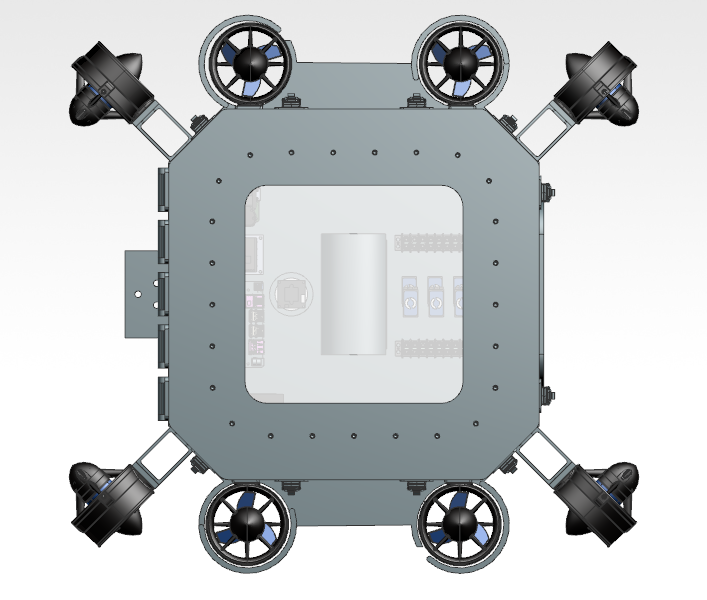
\includegraphics[scale=0.35]{images/sub3.PNG}}
    \caption{CAD of top-view of Erie.}
    \label{fig:sub3}
\end{figure}

 This design made accessing electrical components inside the hull significantly easier because opening the hull only involved undoing the latches and pulling the lid up on its hinges. It also makes it easy to view the status lights of the electrical system without opening the lid which is useful while testing, see figure \ref{fig:sub3}.

To address the maneuverability design criteria, we designed our sub to accommodate eight thrusters instead of the six we had last year. Having this amount of thrusters allowed us to achieve all six degrees of freedom. One of the issues that Huron had was that it would pitch undesirably when moving forwards or sideways. To avoid this issue on the new sub, we designed thruster mounts that would allow the horizontal thrusters to slide up and down. Thus, we could fine-tune the exact positions of the horizontal thrusters in order to make the sub move straight when the thrusters are activated.

One of the strengths of Huron was that it could accommodate some modularity in the sense that new components could be implemented to the sub in the future. To incorporate a similar trait on the new sub, we designed a plate that sits directly below the main hull and contains mounting locations for future sensors, such as a Doppler Velocity Log (DVL), to be mounted. We performed stress analysis on the plate to make it as lightweight as possible without deforming under the large weight of the hull.


\subsection{Electrical}
    \paragraph{Power Distribution}
    With our increasing number of sensors and power usage of our computers, we decided it would be necessary to upgrade our power delivery system. This would not only ensure our current setup could be fully powered but also that future additions would be able to receive sufficient power. Additionally, with a new setup, we could use more secure and consistent connectors throughout our power delivery. For our new power distribution board, we used an off the shelf Pololu 5V 15A Step Down Regulator as our DC-DC converter which would supply up to 75 W to our system. We mounted this to a custom PCB distribution board using the solid Molex MicroFit 3.0 connectors to distribute power to our components, along with some extra slots we could populate later on. 

    \paragraph{Sensor Optimization}
    Last year we used the PixHawk's built-in IMU to measure our orientation. However, this IMU only provides its data message at 20 HZ, and it is difficult to access since it is part of the MAVROS stack. So, we purchased and integrated a Spartan AHRS, which provides data at 30 HZ and is easily accessible over the serial bus. This sensor leverages the AdaptNav\textsuperscript{TM} filtering algorithm to provide quality data. This enabled us to integrate and control our heading much more reliably.
    
    
    We also researched sensors to add to the AUV, particularly a Doppler Velocity Log (DVL) and sonar. Our advisor, Dr. Katherine Skinner, lent us a sonar sensor which we experimented with in-water several times. However, we ultimately decided that we didn't have the bandwidth to add additional sensor systems for this year's AUV given our focus on the computer vision and hydrophone system development.

\subsection{Software}
    \paragraph{Controls and Architecture}
    
    Our system utilizes the Robot Operating System (ROS) framework to facilitate communication between sensors and our navigational algorithms. 

    The largest development to our architecture was the adoption of the state machine pattern. In this pattern, a given ROS node can have some set of states, each with some distinct behavior, and transitions between these states. Explicitly naming and referencing these states in the code allows us to easily reason about the node's behavior. The most prominent usage of this pattern in our code is in the high-level task planning logic. Previously we had a designated ROS node which started each task individually, but we found that this paradigm made it difficult to assess when a task had been successfully completed and when to move onto the next task. Instead, a single node now contains a state machine and performs both the gate and buoy tasks. When completing the Gate Task, the robot will first scan for the gate. Once the gate is seen, the robot will begin to approach the gate. If at any time the robot is sufficiently confident that it cannot see the gate, it will transition back to the scanning state. If instead it sees one of the images on the gate, it will transition to approaching the image. Finally, once it believes it has gotten close to the gate, it will transition to a crossing state. A full state machine diagram, including the transition to the buoy task, can be seen in Appendix A. By breaking the task into distinct phases, we are better able to debug and reason about the robot's behavior. This pattern also serves as a framework for approaching more complex tasks in the future as it allows for the AUV to re-attempt tasks. 
    
    Another aspect of our codebase we sought to streamline was our usage of third-party libraries. We found that directly using the interfaces and boilerplate code of common libraries, such as MAVROS which we use to interface between our flight controller and algorithms, made our code less readable and harder to maintain. To solve this problem, our team wrote ``adaptor" classes to serve as a layer of abstraction to improve readability and maintability of our codebase. One example is a MotorController module to interact with MAVROS. The default MAVROS interface requires setting six values (one for each degree of freedom) in an arbitrary order. Our module, on the other hand, allows us to only name the values we wish to change in any given ROS node, leading to clearer and more declarative code. Another example is the ROS PID library that we use for the various PID controllers used for navigation. The library requires publishers and subscribers on multiple topics, which must be constructed through boiler-plate code. To solve this problem, we wrote an abstraction which allows us to construct all of these in a single line of code and declaratively set parameters as necessary. By making use of abstractions like these, our team is building a strong foundation of readable and maintainable code which can be easily re-used. 
    
    
    \paragraph{Deep Learning}
    This past year we made significant advancements with our deep-learning based object detection systems. We upgraded to the newly released YOLOv5 from the now deprecated Tiny YOLOv3 and implemented real-time detection for multiple different objects. 
    
    YOLOv5, meaning You Only Look Once version 5, is an off-the-shelf machine learning model that was perfect for our needs. It is lightweight and fast, ideal for storing and running in real time for detection on our sub. It also is very easy to train, requiring only labeled images and a configuration file. Our previously used version of this model, YOLOv3, was large and slow to run, only processing around 1 image every 2 seconds. Upgrading to the newer version, along with refactoring the code that analyzes the model's output, allowed us to increase this frame rate to around 5 images per second.
    
    Another reason we upgraded to YOLOv5 this year is that is utilizes the PyTorch framework instead of a framework called Darknet. PyTorch is an open source machine learning framework and is an industry standard for this type of work. It is very easy to use, and its established reputation means that there is lots of helpful documentation and greater usability compared to our previously used framework of Darknet. With this change, we were able to train our models in a different way as well. We now utilize a service called the Great Lakes Computing Cluster for all of the computational power used generating the model. Access to this service was granted from being a University of Michigan group, and it allows us to abstract away the architecture we train on and get our resulting model in a fraction of the time.
    
    An additional important change we implemented was the ability to detect multiple classes of objects. Prior to this year, we only had the ability to detect the gate object. For competition this year, we found it necessary to be able to recognize the gate, bootlegger, G-man, badge, and gun objects to successfully complete the tasks we had in mind. We needed to vastly expand our data set to achieve this, not only adding images for all of the new objects, but also new gate images since our old gate images did not have pictures hanging from the gate like it has this year. Even in past years, we believe the number of images in our data set was too small, over-fitting the model to our test setting. Continuing to expand our data set into thousands of images per object type is still a goal for the future, as our model will perform well in different environments and will be able to detect better from all sorts of angles.
    
    
    % YOLOv5 Creativity Discussion - Andrew: anything else we should add here?
    % - Utilizes pytorch instead of darknet, this makes it more usable -> can train on the cluster now too
    % - Multiple object detection -> this year we added support for detecting multiple classes in real-time, required code base refactoring to recover frame rate
    % - Dataset expansion -> this is the area where we still need the most work in terms of organization but we significantly expanded our dataset to actually include multiple classes and successfully train accurate models
    
    \paragraph{Computer Vision (CV)}
    Additionally, we expanded our computer vision toolkit to use classical CV methods which are generally computationally less expensive than deep-learning models. We applied a Canny edge detection algorithm as well as color threshold masking to detect markers in the pool. The first step of Canny is to smooth the image using a Gaussian kernel, then we convolve the Sobel kernels over the image to get the edge gradients. This on its own does get us the edges, however, after some experimentation, we determined we were reading in too much noise. This is where the rest of the Canny algorithm was helpful. Using the two x and y gradients from the Sobel Kernels, we were able to get the angle of the gradient of each pixel. This is helpful when suppressing the edges so they are thinner. Ideally we should get thin lines for the edges so we are only getting the exact border of the way point. We used a max threshold that filtered pixels by weight, if the edge was deemed strong it was left in the final image. The stages of the edge detection can be seen in Figure \ref{fig:edgedetect} below.
    \begin{figure}[htbp]
    \centerline{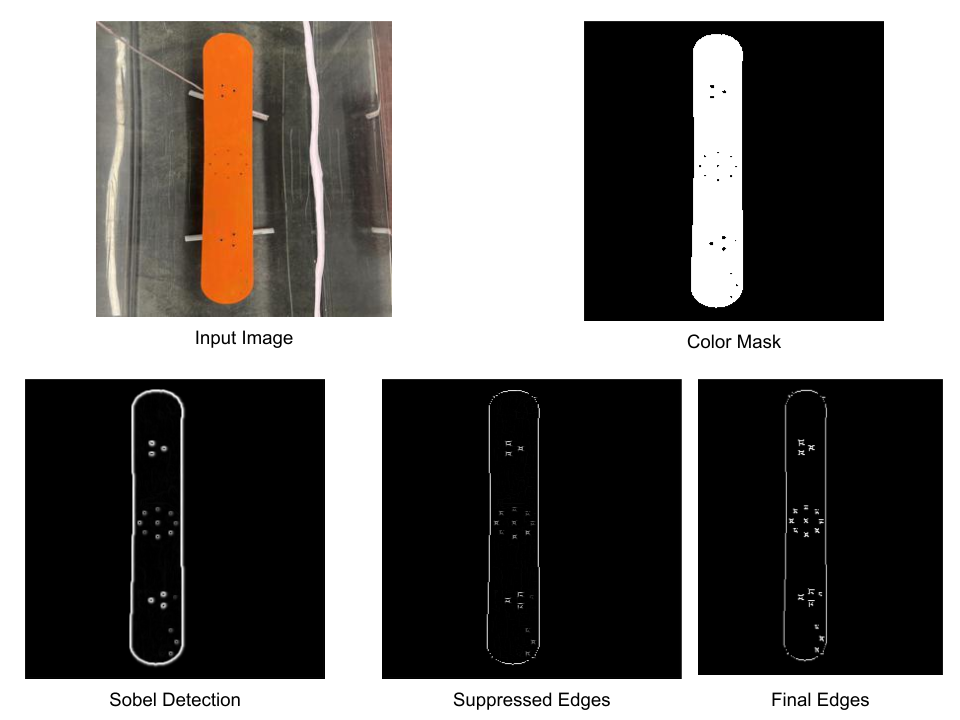
\includegraphics[scale=0.25]{images/Way point Detection Figure.png}}
    \caption{Classical CV path marker detection.}
    \label{fig:edgedetect}
    \end{figure}


\section{Experimental Results}
As the availability of our testing facilities and team members were sometimes limited due to the COVID-19 pandemic, we devised methods to more efficiently develop and test software both on and off the AUV.


    \paragraph{Off-Board Software Testing}
    In order to write, execute, and test our software off of the AUV, we developed Docker images that emulate our companion computer, PixHawk flight controller, and the MAVROS environment. This workflow allows anyone on our team to setup our development environment on their computer in just a few steps. In general, we tested the logic of our software off-board of the AUV and reserved in-water testing for collecting data to improve our vision system or test the physical results of the algorithms once they had been tested in simulation.

    To visualize the output of our software both in Docker and on the real AUV, we created visualizations using RQt, a ROS dashboard library. We leveraged RQt to graph position data and dynamically tune control parameters, allowing for easy incremental testing.
    
    We also developed a Unity simulation that communicates with our software emulation in Docker via the 
    ROS-TCP-Connector package. We wrote Unity C\# software to simulate the movement, sensor data, and vision data of the AUV with noise. The simulation features to-scale competition object models created by Team Inspiration, allowing us to evaluate our software's behavioral logic within the competition environment [1].
    
    \begin{figure}[htbp]
    \centerline{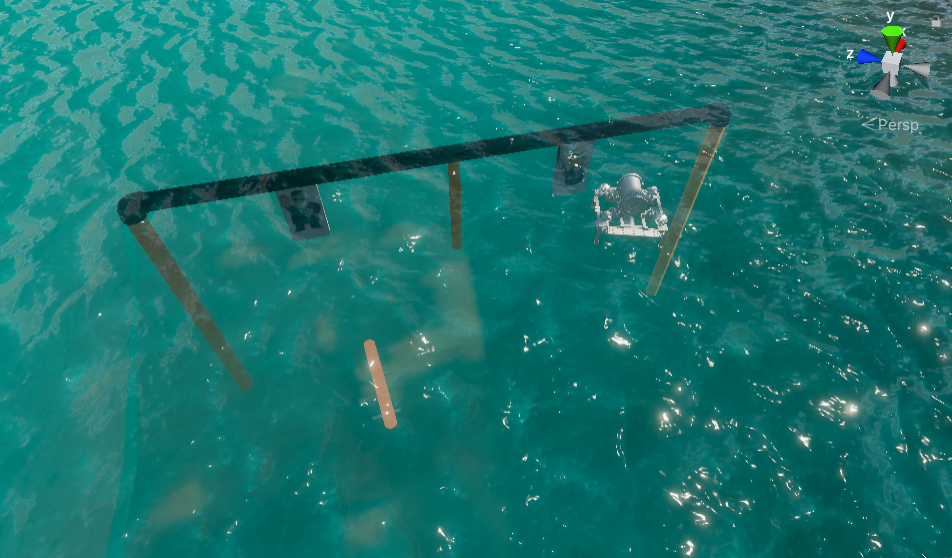
\includegraphics[scale=0.3]{images/unity.png}}
    \caption{Testing the gate task logic using Docker and Unity.}
    \label{fig}
    \end{figure}

    \paragraph{In-water Testing}
    Almost all in-water testing was done at the Marine Hydrodynamics Laboratory (MHL) with smaller tests being completed in a water tank inside of the Ford Robotics Building at the University of Michigan. During testing sessions, the AUV was connected to our base-station using an ethernet tether, allowing us to easily edit code or change tests. During the school semester, we had about one day per week in which we were able to test inside of the MHL, this number increasing once the semester had ended and students were available more frequently. Before each testing session, test plans were premade and followed to promote a productive use of time. The value that was placed on each task in the plan was ultimately situational, depending on what the team felt was most necessary at the time. In addition, various programs were written that tested specific functions and systems. These test-programs were often very simple and pretested in the water tank at the Ford Motor Company Robotics Building to ensure progress at the MHL. Examples of these programs include basic depth control, in-water stability, and orientation control. It is worth noting that, while these programs were written to be simple and easily adjusted, they were necessary to the functionality of the submarine. For example, stability control was the most problematic, which took a large amount of effort to incorporate. While we were able to ignore this program in many of the tasks, it was also necessary to finish because the testing submarine had an awkward natural orientation, which disrupted its path over long distances. In contrast, most task programs were tested with both the depth and orientation controls engaged because of their higher consistency. After the end of the school year, there has also been a shift in the testing requirements due to our competition submarine body being finished. This meant that the problems we experienced on our testing sub were now less exaggerated.
    \paragraph{Deep Learning Model Training}
    
    Last year our object detection testing focused primarily on developing a system that could perform in any underwater condition regardless of lighting and background color. This year with the introduction of four additional classes that we could identify and continuing to utilize our gate data set from last year, it did not make sense to compare our previous models to this years. Instead as we expanded our data set throughout the year we examined the accuracy of our model on a predefined test set containing complex situations like the ones seen in figures \ref{fig:buoys} and \ref{fig:gate}.
   
    \begin{figure}[htbp]
    \centerline{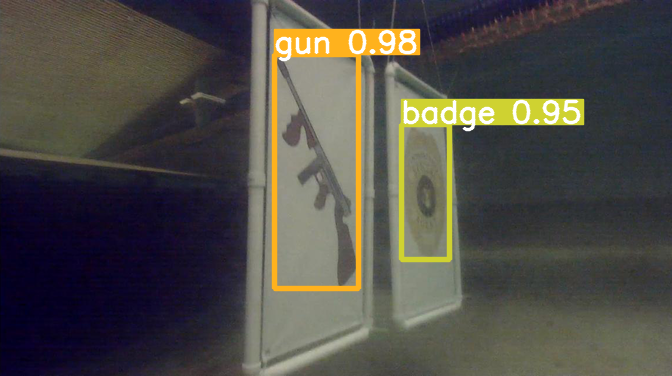
\includegraphics[scale=0.3]{images/11222021_672_376_181.png}}
    \caption{Buoy inference output from YoLo v5 model.}
    \label{fig:buoys}
    \end{figure}
    \begin{figure}[htbp]
    \centerline{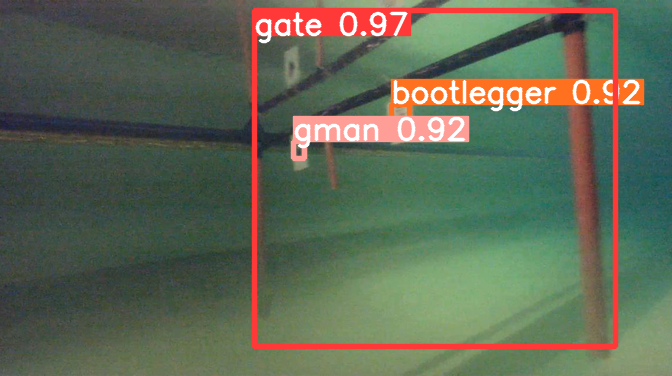
\includegraphics[scale=0.3]{images/11222021_672_376_477.png}}
    \caption{Gate inference output from YoLo v5 model.}
    \label{fig:gate}
    \end{figure}
    
    To train machine learning models faster so that the recent model parameter changes could be observed  quickly, we switched from training models on Google Colab to doing so on a high performance computing cluster called the Great Lakes Cluster. The initial upload and subsequent updates of the training data, test images, and the Yolov5 program were automated through a script using git version control and Linux permission commands. The label creation and organization was handled by a Python script that reads a Labelbox export file.

    Additionally, the machine learning model training process on the Great Lakes Cluster was automated using a series of scripts. These scripts initialized a Python virtual environment, installed dependencies for Yolov5, initiated PyTorch for Yolov5 inferencing, and read and handled Yolov5 machine learning model arguments from the designated text file. Using the proper arguments and Yolov5, the scripts trained the machine learning model, ran inferencing, converted weights, and dynamically organized Yolov5’s end weights, model evaluations, and results. After, Globus was utilized to transfer result and weight files to a laptop for submarine usage.

    Furthermore, the Slurm Workload Manager framework was utilized to allocate the proper number of threads, GPU, and CPU memory for training the machine learning model. We also incorporated the option to utilize Slurm’s job arrays, which allows for models with different parameters to be trained concurrently for efficient model comparison. The output and error logs were stored in a dynamic sectioned file logging system that also supports multiple logs from job arrays. 

    By training models on a high performance computing cluster, not only was file management easier and the training processes streamlined outside of the abnormal Google Colab environment, but models could be trained at the same time, and each was trained $324\%$ faster than if it were to be trained on Google Colab.
 
\section*{Acknowledgements}

The Michigan Robotic Submarine team would like to thank our sponsors for their monetary support: University of Michigan College of Engineering and Ford Motor Company. In addition, we would like to thank our advisor Dr. Katie Skinner for continuously supporting our team by advising us and providing a generous workspace and testing area to use freely. 

We are greatly appreciative of the Marine Hydrodynamics Lab staff, especially Jason Bundoff, for graciously providing the team with an in-water testing location. We also would like to thank the Wilson Student Team Project Center facilities and Ford Motor Company Robotics Building staff for hosting our team workspace, providing tools and resources, and overall supporting our endeavors. 

We are also thankful for the hydrophone and image data provided through the RoboNation data sharing program.

\begin{thebibliography}{00}
\bibitem{b1} Inspiration Robotics, "RoboSub-Simulation". Github.com. https://github.com/InspirationRobotics/RoboSub-Simulation (accessed June 11, 2022)
\bibitem{b2} A. Zelenak, "A PID controller for ROS". bitbucket.org. https://bitbucket.org/AndyZe/pid/src/master/ (accessed June 11, 2022)
\bibitem{b3} ]G. Jocher, “ultralytics/yolov5: v6.1 - TensorRT, TensorFlow Edge TPU and OpenVINO Export and Inference”. Zenodo, Feb. 22, 2022. doi: 10.5281/zenodo.6222936.

\end{thebibliography}

\clearpage
\appendices
\section{Task State Machine} % TODO

\vspace{0.5cm}
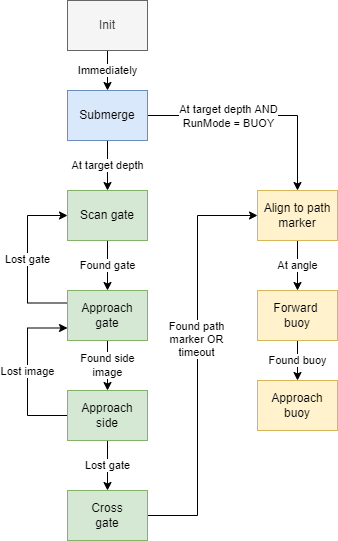
\includegraphics[scale=0.6]{images/task_state_machine.png}
\newpage


\section{Outreach Efforts}
Michigan Robotic Submarine assisted the University of Michigan's Department of Naval Architecture and Marine Engineering (NAME) with their annual SeaPerch competition for middle and high schoolers in the greater Ann Arbor area in March. The team showcased our work, talked to students, and helped with running the event. 

In the future, we plan to assist with this event as well as other outreach events through the NAME department.

Additionally, we participated in the RoboNation Data Sharing committee with one of our members joining the initial group. Through piloting the program, we provided feedback and input on the program and how it would provide the best value to teams.


\clearpage
\section{Component Specifications}
\begin{table}[htbp]
\begin{center}
\begin{tabularx}{\textwidth}{|X|X|X|X|X|X|}
    \hline
        Component & Vendor & Model/Type & Specs & Cost (if new) & Year of Purchase \\ \hline
        Buoyancy Control & Blue Robotics & R-3312 Subsea Buoyancy Foam & N/A & \$135.00 & 2022 \\ \hline
        Hull  & American Tooling \& Prototype & Custom & 6061 Aluminum & \$3250.00 & 2022 \\ \hline
        Cable Penetrators & Blue Robotics & Potted cable penetrators & 25mm long M10x1.5 for 6mm cable & \$120.00 & 2020 \\ \hline
        Thrusters  & Blue Robotics & T200 w/ Propellor & 7-20V & \$1,074.00  & 2020\\ \hline
        Thruster Mounts  & Custom & N/A & 6061 Aluminum & N/A & N/A \\ \hline
        Motor Control  & Blue Robotics & Basic ESC & 7-26V & \$172.00  & 2022 \\ \hline
        High Level Control  & Custom & Captain & ROS-based & N/A & N/A \\ \hline
        Battery  & Blue Robotics & Lithium-ion Battery & 14.8V, 18Ah & \$350.00  & 2022 \\ \hline
        Converter  & N/A & N/A & N/A & N/A & N/A \\ \hline
        Regulator & Pololu & Step-Down Voltage Regulator & 5V, 15A & \$59.95 & 2022 \\ \hline
        CPU & Nvidia & Jetson Nano & Quad-core ARM A57 @ 1.43 GHz, 4 Gb RAM & \$110.00  & 2021 \\ \hline
        ~ & RaspberryPi & Raspberry Pi 3B & 1.4GHz 64-bit quad-core, 1Gb RAM & \$35.00  & 2020 \\ \hline
        Internal Comm Network & Open Robotics & ROS Kinetic & ~ & N/A & N/A \\ \hline
        External Comm Interface & - & Ethernet & - & - & N/A \\ \hline
        Compass  & PixHawk & PX4 & Accel/Gyro: ICM-20689 with Magnetometer & \$257.00  & 2020 \\ \hline
        Inertial Measurement Unit (IMU)  & PixHawk & PX4 & MPU6000 9-axis & (see above) & (see above) \\ \hline
        Doppler Velocity Log (DVL) & N/A & N/A & N/A & N/A & N/A \\ \hline
        Vision & Stereolabs & ZED2 & stereo vision, ROS, depth detection & \$449.00  & 2020 \\ \hline
        Acoustics & Aquarian Audio & H1C Hydrophone & omnidirectional, no amplifier & \$139.00  & 2021 \\ \hline
        Algorithms: vision  & N/A & miniYOLOv3 & used to train convolutional neural network & N/A & 2022 \\ \hline
        Algorithms: acoustics  & N/A & custom (see Hydrophone - algorithms section) & N/A & N/A & N/A \\ \hline
        Algorithms: localization and mapping  & N/A & N/A & N/A & N/A & N/A \\ \hline
        Algorithms: autonomy  & N/A & Custom & N/A & N/A & N/A \\ \hline
        Open source software & N/A & OpenCV & Computer Vision & N/A & N/A \\ \hline
        Open source software & N/A & Andy Ze ROS PID & PID Control & N/A & N/A \\ \hline
    \end{tabularx}
\label{tab1}
\end{center}
\end{table}




\end{document}
